\documentclass{acmart}
\usepackage{amsthm}
\usepackage{amsmath}
\usepackage{amsfonts}
\usepackage{amssymb}

\title{Report for HW 1 in CSC 240}

\author{Sailesh Kaveti}

\begin{document}

\maketitle

\section*{Introduction}

For this assignment, we were asked to analyze a data set of our choice and compute some statistics and plot data. For this assignment, I used Python to generate the charts. To help me with this, I used the following Python libraries: NumPy, Pandas, and Matplotlib.pyplot. With regards to the dataset, I used a baseball dataset taken from the Rotowire website for the 2018 season and cleaned up manually in Excel. In general, the baseball dataset includes 27 different statistics about each of the players, each of which has some significance. I placed this data into a CSV file, and loaded this data into a dataframe object using Pandas. For the analysis of the data, I generated four different charts that will be discussed below. The four charts are HRs vs. SLG, Hits vs. AVG., Age vs. OPS, and Age vs. Strikeouts.

\section*{Hits vs. AVG.}

\begin{figure}[H]
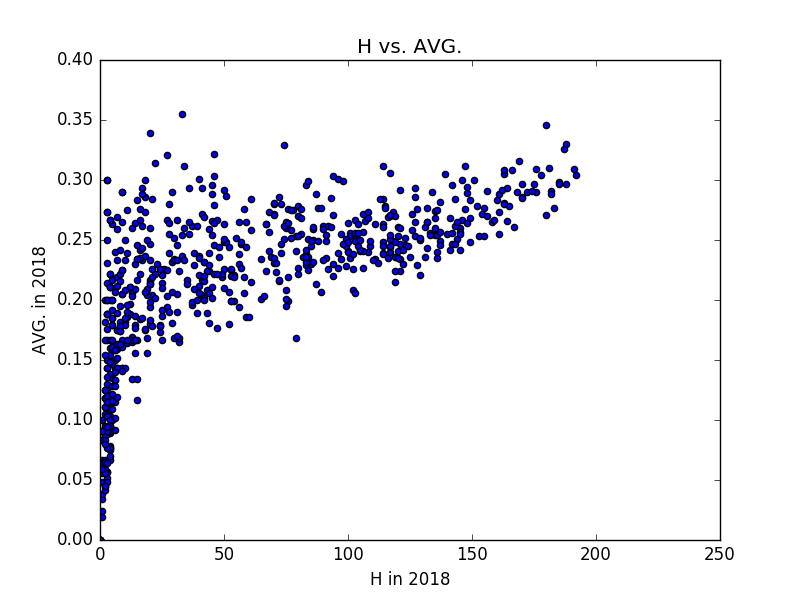
\includegraphics[scale=.5]{HvsAVG.png}
\end{figure}

Hits (H) and Average (AVG) are two simple but informative statistics in Baseball. The AVG is computed with the following formula: 
$$
SLG = \frac{H}{AB}
$$
Upon looking at the formula for AVG, the relationship between H and AVG is clear and should be reflected in the chart. However, if a player has only a few AB, then their H total could be low while still allowing the AVG to be high. That being said, I thought it would be interesting to plot the relationship between the two. There is a positive correlation between H and AVG, meaning that as the number of hits a person has, it is likely that their AVG increases.

\section*{HRs vs. SLG}
\begin{figure}[H]
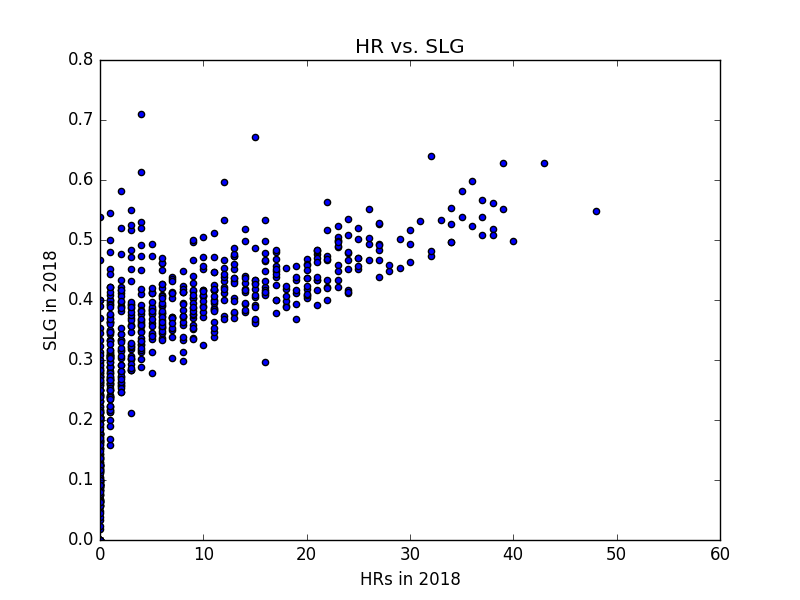
\includegraphics[scale=.5]{HRvsSLG.png}
\end{figure}
Homeruns (HR) and Slugging (SLG) are two very important statistics in Baseball. While HR is a rather self explanatory statistic, SLG is computed by the following formula:
$$
SLG = \frac{H + 2B + 2 * 3B + 3 * HR}{AB}
$$
As seen, the relationship between HR and SLG is rather direct, so I plotted a scatter plot to see if I could indeed see a correlation between the two. In the chart, it is rather clear that the equation is indeed well reflected, as there is a positive correlation between HR and SLG. As the number of HRs that a person hits increases, it is likely that their SLG also increases.

\section*{Age vs. Average OPS}

\begin{figure}[H]
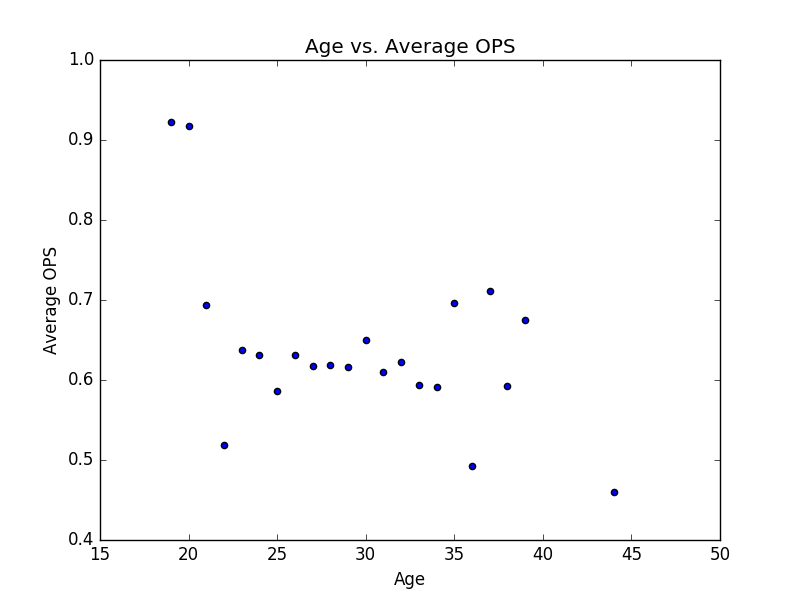
\includegraphics[scale=.5]{AgevsAverageOPS.png}
\end{figure}

Using my dataframe object, I called the GroupBy command in order to properly group the data by each age and took the average of the On Base Percentage (OBP) plus Slugging (OPS) statistic. For reference, the OPS statistic is calculated with the formula:
$$
OPS = \frac{H + BB + HBP}{AB + BB + HBP + SF} + SLG
$$
In short, this statistic is one of the best representations of how good a player is, allowing for a holistic evaluation for each player. Looking at the graph, as the  player gets older, their OPS goes down, meaning that their total performance as a player decreases overtime. This is a negative correlation. There is one very clear explanation for this. As a player gets older, the slower and less powerful they become, decreasing both the OBP and SLG statistic. They are also more likely to get reduced playing time as their body goes through more wear and tear. That being said, there are certainly some outliers that need to be accounted for. At both extremes of the chart (19-21 and 36-44), there are very few players, meaning that a player that is in that age group are likely to heavily influence the average for that age.

\section*{Age vs. Average SO}

\begin{figure}[H]
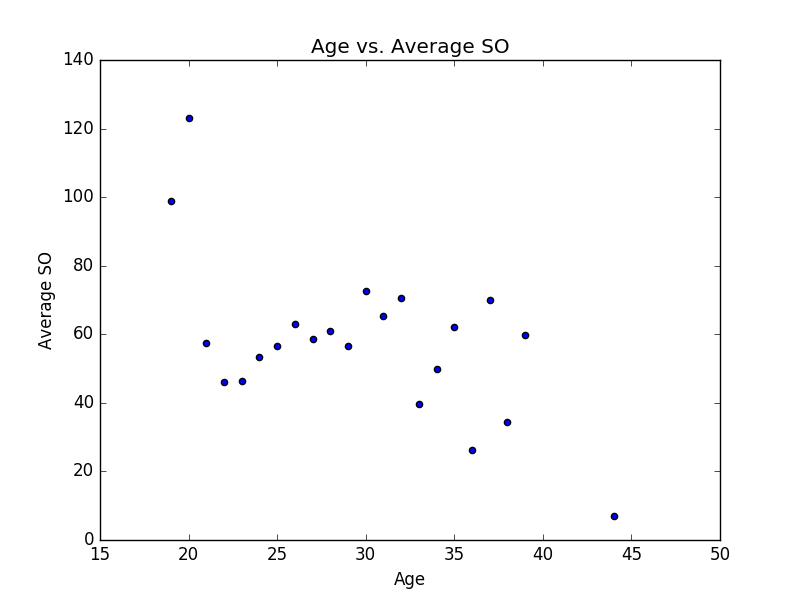
\includegraphics[scale=.5]{AgevsAverageSO.png}
\end{figure}
Similarly to the previous section, I called the GroupBy command to properly group the data by each age and took the average of the Strikeouts (SO) that each player. A strikeout is when the player misses the ball three times in an At Bat (AB). Before I generated this graph, I expected that the SOs would decrease as a person got older because they would have a better knowledge of the game, leading to better discipline when hitting. However, this was not the case, as there was a positive correlation between Age and SOs. The reasoning for this must be similar to the previous section. As a person gets older, the less likely that they are able to keep up with the 90+ MPH pitches because their reflexes and strength decrease. As discussed in the previous section, at the extremes of the chart, there are only a few players, leading to fluctuations in the data. However, there still remains a positive correlation between the ages of 20 - 33.

\begin{thebibliography}{200}

\bibitem{savefig} I learned how to save a PNG from here: \url{https://stackoverflow.com/questions/41204128/attributeerror-module-object-has-no-attribute-save-matplotlib}

\bibitem{scatter} I learned how to create a scatter plot from this link: \url{https://www.youtube.com/watch?v=yejsG6TKWNU}

\bibitem{clear} This is where I learned to clear the chart: \url{https://stackoverflow.com/questions/32801990/how-to-clear-all-dynamically-plotted-points-on-pyplot-scatter-graph}

\bibitem{acmlatex} This is where I downloaded the ACM package: \url{https://www.acm.org/publications/authors/submissions}

\bibitem{groupby} This is where I learned how to use the Group By function: \url{https://www.shanelynn.ie/summarising-aggregation-and-grouping-data-in-python-pandas/}

\bibitem{reset} This link is where I learned how to reset the index to better use the Group By function: \url{https://stackoverflow.com/questions/39494246/how-to-plot-data-after-groupby}

\bibitem{documentacm} This is where I found documentation for the ACM: \url{https://www.acm.org/binaries/content/assets/publications/consolidated-tex-template/acmart.pdf}

\bibitem{stats} This is where I got my data from: \url{https://www.rotowire.com/baseball/stats.php}

\bibitem{NumPy} The documenation for NumPy can be found here: \url{https://docs.scipy.org/doc/}

\bibitem{Pandas} The documentation for Pandas can be found here: \url{https://pandas.pydata.org/pandas-docs/stable/reference/index.html}

\bibitem{Matplotlib} The documentation for Matplotlib.pyplot can be found here: \url{https://matplotlib.org/api/_as_gen/matplotlib.pyplot.html}

\end{thebibliography}

\end{document}